\chapter{Real-Robot Experiment}\label{ch:real_robot_experiment}

After investigating the research problems in simulation, this thesis continues to conduct the experiments on a real robotic system. In \cref{sec:real_robot_experiment:experiment_setup}, the setup for the real-robot experiment is described in details. The results are presented and analyzed in \cref{sec:real_robot_experiment:results_and_discussion}.

\section{Experiment Setup}\label{sec:real_robot_experiment:experiment_setup}

This section


\subsection{Hardware setup}

Unlike the simulation experiments, described in \cref{ch:simulation}, the real-robot experiment uses two separate computers for the \gls{amr}'s onboard system and the edge computer. For the robot, the onboard system uses a \gls{nuc} equipped with an Intel(R) Core(TM) i3-8109U \gls{cpu}, which is commonly used for \glspl{amr}.  For the edge, a \gls{linux} desktop computer equipped with an Intel(R) Core(TM) i3-8109U \gls{cpu} and a Nvidia GeForce GTX 1060 6GB \gls{gpu} is used. On both computers, the offloading module and the perception modules have full access to the available resources. The distribution of the modules between the two computers is illustrated in \cref{fig:real_robot_experiment_setup}. The \gls{ros} bag replay of the simulated scenario is carried out on the robot. The output data of the metrics are also recorded on the robot. The edge computer is solely responsible for the inference of the offloaded images and monitoring the edge system states and sending them to the robot. The image inference is computed by the \gls{gpu} on the edge computer with help of \gls{pytorch} library, while the image inference on the robot is computed by its onboard \gls{cpu}. As mentioned in \cref{sec:general_setup:evaluation}, the system states of the robot and the edge are measured with the "system status" package.

% TODO: add a photo of nuc is this figure
\begin{figure}
    \centering
    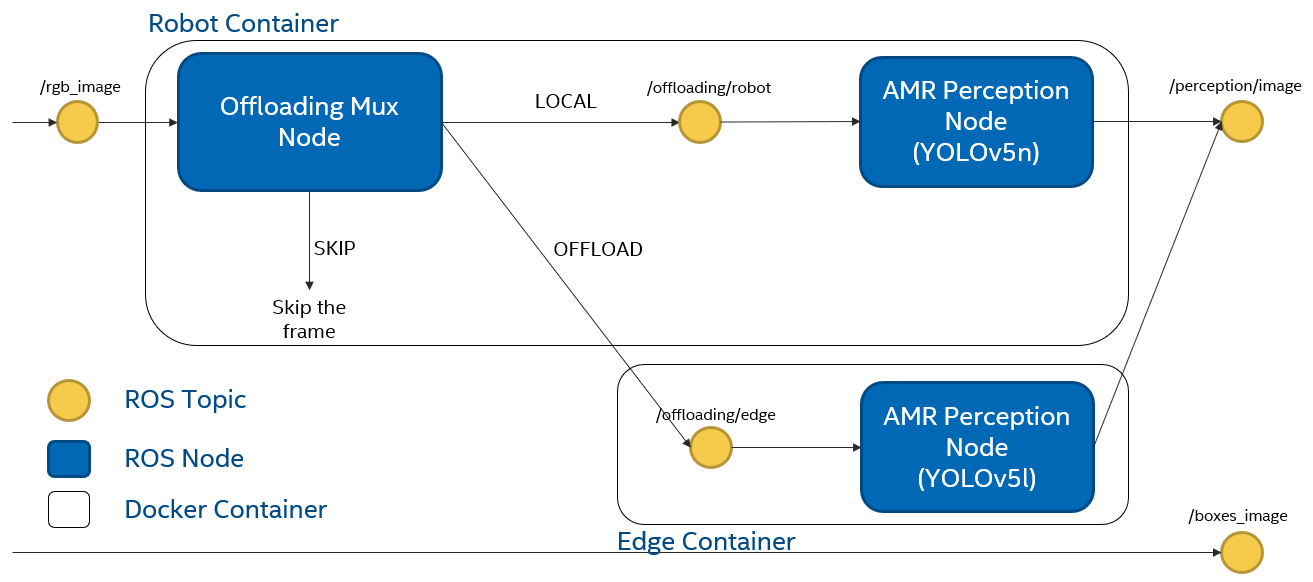
\includegraphics[width=\linewidth]{figures/setup/general_setup.png}  % TODO: change here
    \caption{Setup for real-robot experiment (TODO: adapt this fig)}  % TODO: change here
    \label{fig:real_robot_experiment_setup}  % TODO: change here
\end{figure}


\subsection{Network setup}

Two network interfaces are used to conduct the real-robot experiments. First, the experiment uses an Ethernet connection between the two computers. Similar to the simulation experiments, two network conditions are tested under the Ethernet connection. First, an Ethernet network interface without bandwidth constraints is used to simulate a perfect network connection between the robot and the edge. Then, the Ethernet network interface is constrained to 160 Mbits/s bandwidth to simulate a bag network connection. Finally, a \gls{wifi} network interface is used the carry out the experiment. The \gls{wifi} network has unstable network bandwidth from time to time and therefore affects the experiment results drastically. This is to investigate different offloading strategies under dynamic network condition changes. When conducting the experiment with one network interface, the other one is shutdown to avoid the offloading pipeline uses both network interfaces simultaneously. 

Similar to simulation experiment, \gls{fast_dds} is used as middle ware for \gls{ros}.The \gls{qos} reliability policy for offloading is set to "best effort" and the publishing mode of \gls{fast_dds} is set to asynchronous to avoid the publisher blocked by the network. Moreover, the queuing settings use "keep last" policy and the queue size is set to five messages. Under various \gls{qos} settings, this setup achieves the best performance of the object detection task. However, other \gls{qos} settings are also investigated during the experiments. In \cref{ch:appendix_a}, the results of the experiment with "reliable" reliability policy are presented. 

% Template for single figure

\section{Results and Analysis}\label{sec:real_robot_experiment:results_and_discussion}

The results of the metrics using the Ethernet are shown from \cref{fig:real_robot_experiment:eth_map} to \cref{fig:real_robot_experiment:eth_bandwidth}. In \cref{fig:real_robot_experiment:eth_map}, the \gls{map} under two network conditions are shown. In \cref{fig:real_robot_experiment:eth_rtt}, the \gls{rtt} of the robot perception and the edge perception under two network conditions are shown. \Cref{fig:simulation:execution_time_160} and \cref{fig:simulation:execution_time_320} break down the \gls{rtt} into two components: inference time and network latency and show the results under two network conditions separately. In \cref{fig:real_robot_experiment:eth_overall_processed_frame_percentage}, it shows how much percentage of all the images are processed by the perception modules. \Cref{fig:real_robot_experiment:eth_processed_frame_percentage_160} and \cref{fig:real_robot_experiment:eth_processed_frame_percentage_320} break down the results in \cref{fig:real_robot_experiment:eth_overall_processed_frame_percentage} into two components and show how much percentage of all the images are processed by the edge computer and the \gls{amr}'s onboard system. In \cref{fig:real_robot_experiment:eth_cpu_percentage}, \cref{fig:real_robot_experiment:eth_cpu_energy_consumption}, and \cref{fig:real_robot_experiment:eth_bandwidth}, the \gls{cpu} usage, the \gls{cpu} power consumption and the network bandwidth usage of the \gls{amr}'s onboard system under two network conditions are shown respectively. 

% #######################################
\subsection{Ethernet without bandwidth constraints}
% #######################################

When the network condition is not constrained, the "edge only" strategy shows the best results in the object detection task, as shown in \cref{fig:real_robot_experiment:eth_map}. This is mainly caused by two reasons. On one hand, the edge computer is using the more complex network, i.e., \gls{yolov5}l, which provides a more precision detection. On the other hand, even though the \gls{rtt} of the edge perception is still higher than the robot perception, the difference is still relatively low, as shown in \cref{fig:real_robot_experiment:eth_rtt}. Therefore, the inaccuracy caused by the execution delay is negligible. Moreover, the "edge only" strategy also processed the most frames in the experiments. This also makes the "edge only" strategy the safest among different strategies. With more detection frames, the \gls{amr} is able to adapt its behavior to the detection more quickly. The "edge only" strategy also uses the least \gls{cpu} and energy of the onboard system, since the images are exclusively calculated on the edge computer. This is beneficial to \gls{amr}'s onboard system and battery life. This also allows the \glspl{amr} to free up more resources for other tasks, e.g., \gls{slam}, navigation, and path planning. However, the "edge only" strategy also uses the most network bandwidth. For image feed with 30 \gls{fps} at a resolution of 848x640 pixels, around (TODO: add a number here) MB/s bandwidth is used for offloading. Such bandwidth will be a huge amount for wireless connection. For comparison, IEEE IEEE 802.11ac (\gls{wifi} 5G) can support only up to (TODO: add a number here) bandwidth. If the number of the \glspl{amr} scales, the network cannot provide such bandwidth. Therefore, "edge only" strategy is not suitable for industrial usage. 

% Figure for eth mAP
\begin{figure}
    \centering
    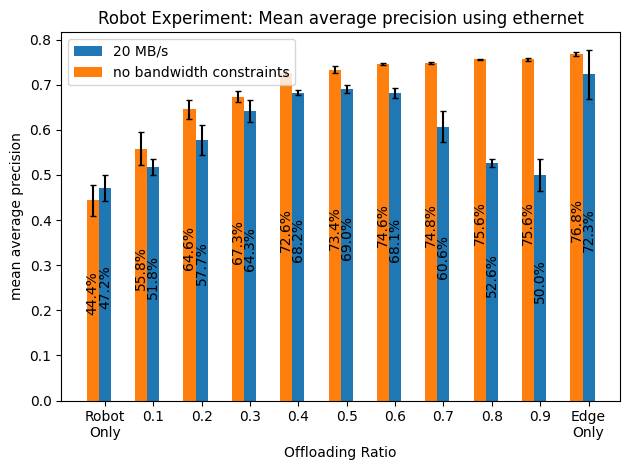
\includegraphics[width=\linewidth]{figures/experiment/real_robot/eth/map.png}
    \caption{Real-robot experiment: \gls{map} with Ethernet}
    \label{fig:real_robot_experiment:eth_map}
\end{figure}

On the other hand, the "robot only" strategy delivers the worst results in the object detection task. This is mainly because the onboard resources are not enough for the \gls{amr} to process all the images. The robot perception module is strained when more images are calculated locally on the \gls{amr}'s onboard system. As shown in \cref{fig:real_robot_experiment:eth_rtt}, the robot perception has the highest \gls{rtt} with "robot only" strategy. The \gls{rtt} of robot perception is broken down to different components in \cref{fig:real_robot_experiment:eth_execution_time_320}. The inference time of the robot perception stays the same. However, the network delay is increased. This indicates that the robot perception module has too many images waiting for processing and the images start to queue, causing the network latency of robot perception to increase. As shown in \cref{fig:real_robot_experiment:eth_execution_time_320}, the network latency of robot perception stabilizes around 0.6 offloading ratio. This infers that the \gls{amr}'s onboard system, i.e., the \gls{nuc}, is only able to process less than 40 percent of the offloaded images, i.e., around 12 \gls{fps}. This corresponds to the 99.9 ms \gls{rtt} of the robot perception at offloading ratio 0.6, as shown in \cref{fig:real_robot_experiment:eth_rtt}. Naturally, the "robot only" strategy also uses the most \gls{cpu} and energy, since it computes the all images onboard, as shown in \cref{fig:real_robot_experiment:eth_cpu_percentage} and \cref{fig:real_robot_experiment:eth_cpu_energy_consumption}. Moreover, the "robot only" strategy uses the least network bandwidth. It still uses 0.4 MB/s network bandwidth because the states monitors need to send system state data from the edge computer to the \gls{amr}'s onboard system.

As illustrated in \cref{fig:real_robot_experiment:eth_map}, the \gls{map} of the object detection task saturates between offloading ratios 0.5 and 0.8. This indicates that both the robot perception and the edge perception are working under their optimal workload. The task performance reaches a stationary point. After the stationary point, the edge perception becomes more prominent for the performance. Therefore, the performance continues to improve due to the more accurate object detection of the more complex model on the edge. 

The decision-making strategy also delivers decent results for the object detection task under good network condition. As shown in \cref{fig:real_robot_experiment:eth_processed_frame_percentage_320}, the decision-making strategy offloads most images to the edge computer and only computes (TODO: add a number here) on the \gls{amr}'s onboard system. This decision can be justified by the low \gls{rtt} of the edge computer. (TODO: add analysis after getting the results). It it worth noticing that decision-making strategy calculates a small portion of the images locally on the onboard system, since the \gls{rtt} of edge perception can increase temporarily due to dynamic changes in the network. However, because the network condition is good, most of the images are offloaded to the edge computer. 

% Figure for eth RTT
\begin{figure}
    \centering
    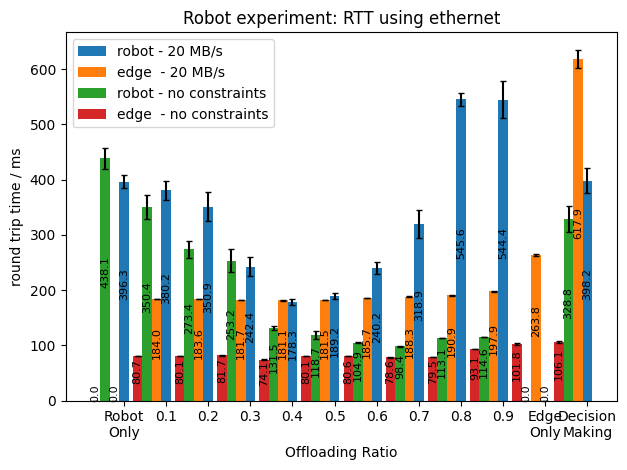
\includegraphics[width=\linewidth]{figures/experiment/real_robot/eth/RTT.png}
    \caption{Real-robot experiment: \gls{rtt} with Ethernet}
    \label{fig:real_robot_experiment:eth_rtt}
\end{figure}

\subsection{Ethernet with constrained bandwidth}

When the network condition is constrained, the "edge only" strategy does not provide the best \gls{map} among all strategies. Since the network is not capable of transmitting the amount of data the strategy needs, the messages starts to queue and the "best effort" reliable policy allows the middleware to drop many messages. This can be visualized in \cref{fig:real_robot_experiment:eth_execution_time_160} and \cref{fig:real_robot_experiment:eth_processed_frame_percentage_160}. The processed frame percentage starts to drop drastically after the offloading ratio exceeds 0.5 and the network latency of the edge perception increases. This also corresponds to the network bandwidth in \cref{fig:real_robot_experiment:eth_bandwidth}. The network bandwidth is at its capacity after the offloading ratio exceed 0.5. Furthermore, with the offloaded images hogging the network bandwidth, it is unlikely for the \glspl{amr} to transmit other data over the network, which can be essential for the safety of the \glspl{amr}. This makes "edge only" strategy the worst strategy under constrained network condition. 

On the other hand, the "robot only" strategy delivers similar results under the two network conditions. Since the "robot only" strategy compute the object detection locally on the onboard system, the performance should be independent from the network conditions. However, it is worth noticing that the there is a slight performance drop for all strategies up to offloading ratio 0.5 due to a slight increase of the network latency on the robot perception. It is suspected that the \gls{netem} layer affects the \gls{ros} middleware and thus causes a increased latency in transmitting the data between the offloading module and the robot perception module. 

The best performance of \gls{map} occurs around offloading ratio of 0.5. At this offloading ratio, the network bandwidth has not exceeded its limits and the robot perception is able to process the given workload. Therefore, the \glspl{rtt} of both perception modules are low and the \gls{amr} is able to get the detection in time. Moreover, offloading at this ratio also allows the \gls{amr} to use less onboard resource, as shown in \cref{fig:real_robot_experiment:eth_cpu_percentage} and \cref{fig:real_robot_experiment:eth_cpu_energy_consumption}. Therefore, under constrained network condition, offloading a portion of the images is the best strategy. However, the offloading ratio is dependent on the available network bandwidth and the computation capabilities of the \gls{amr}'s onboard system.

% Under constrained network condition, the decision-making strategy also managed to deliver decent results. The increased \gls{rtt} time forces the \gls{amr} to compute most of the images locally. However, the decision-making strategy still offloads a portion of the images to the onboard system, because the onboard system is not able to process all images and \gls{rtt} of the robot perception will increase drastically if the images start to queue. These results show that the decision-making strategy is able adapt to the dynamic changes of the network by simply using the \gls{rtt} as a criterion. Furthermore, the \gls{amr} uses more \gls{cpu} and energy with the decision-making strategy under constrained network condition compared to unconstrained network condition, since the \glspl{amr} have to do more computation on the board system and thus consume more onboard resources, as shown in \cref{fig:real_robot_experiment:eth_cpu_energy_consumption} and \cref{fig:real_robot_experiment:eth_cpu_percentage}.

% Figure for eth execution time 160M
\begin{figure}
    \centering
    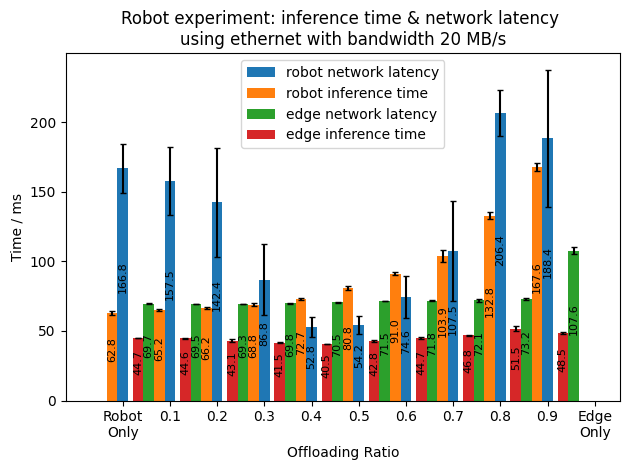
\includegraphics[width=\linewidth]{figures/experiment/real_robot/eth/execution_time_160.png}
    \caption{Real-robot experiment: execution times with Ethernet with 160 Mbits/s bandwidth}
    \label{fig:real_robot_experiment:eth_execution_time_160}
\end{figure}

% Figure for eth execution time 320M
\begin{figure}
    \centering
    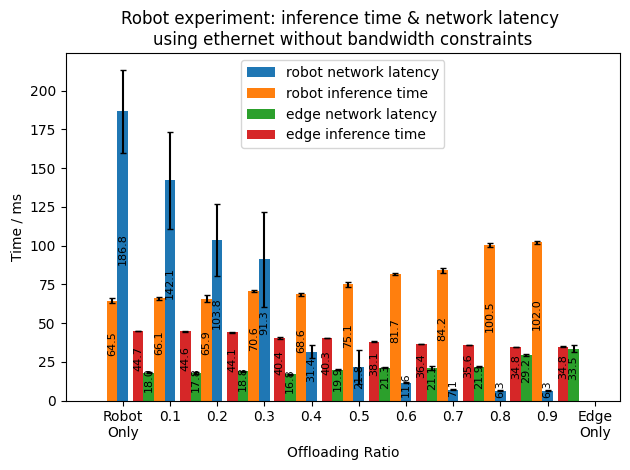
\includegraphics[width=\linewidth]{figures/experiment/real_robot/eth/execution_time_320.png}
    \caption{Real-robot experiment: execution times with Ethernet with 320 Mbits/s bandwidth}
    \label{fig:real_robot_experiment:eth_execution_time_320}
\end{figure}

% Figure for eth overall processed image percentage
\begin{figure}
    \centering
    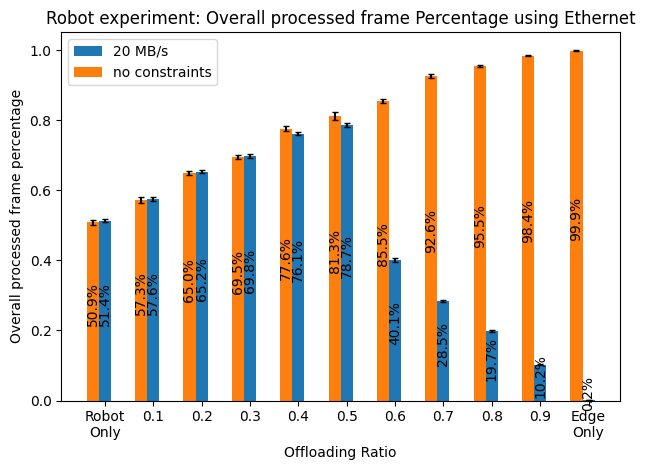
\includegraphics[width=\linewidth]{figures/experiment/real_robot/eth/overall_processed_frame_percentage.png}
    \caption{Real-robot experiment: overall processed frame percentage with Ethernet}
    \label{fig:real_robot_experiment:eth_overall_processed_frame_percentage}
\end{figure}

% Figure for eth processed image percentage 160M
\begin{figure}
    \centering
    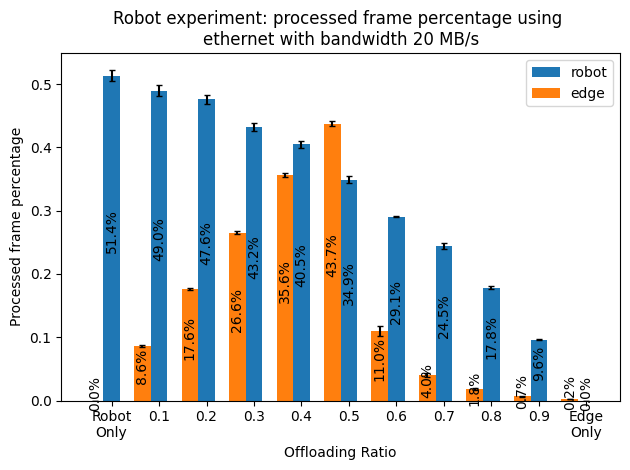
\includegraphics[width=\linewidth]{figures/experiment/real_robot/eth/frame_percentage_160.png}
    \caption{Real-robot experiment: processed percentage with Ethernet with 160 Mbits/s bandwidth}
    \label{fig:real_robot_experiment:eth_processed_frame_percentage_160}
\end{figure}

% Figure for eth processed image percentage 320M
\begin{figure}
    \centering
    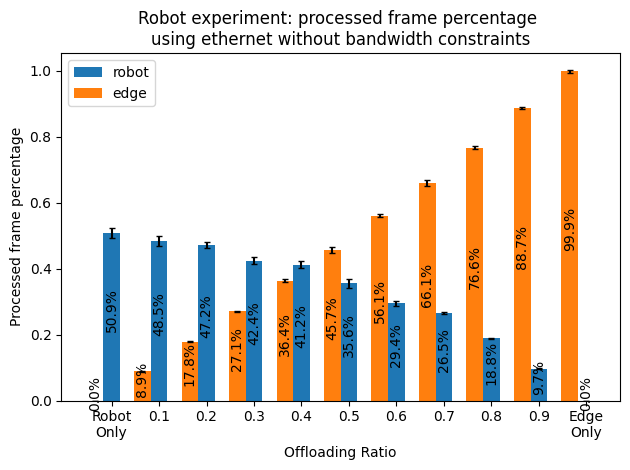
\includegraphics[width=\linewidth]{figures/experiment/real_robot/eth/frame_percentage_320.png}
    \caption{Real-robot experiment: processed percentage with Ethernet with 320 Mbits/s bandwidth}
    \label{fig:real_robot_experiment:eth_processed_frame_percentage_320}
\end{figure}

% Figure for CPU percentage
\begin{figure}
    \centering
    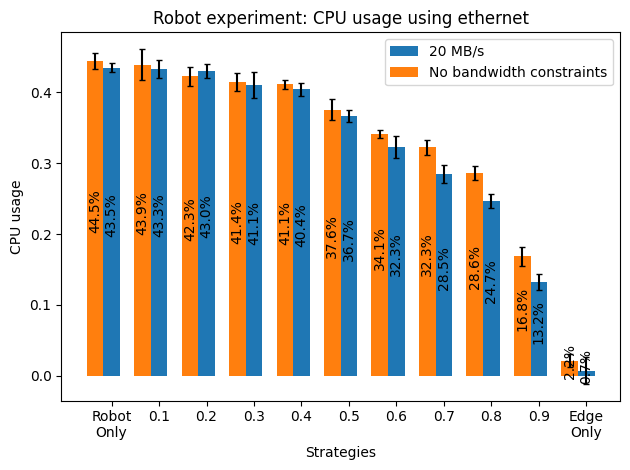
\includegraphics[width=\linewidth]{figures/experiment/real_robot/eth/cpu_percentage.png}
    \caption{Real-robot experiment: CPU usage using Ethernet}
    \label{fig:real_robot_experiment:eth_cpu_percentage}
\end{figure}

% Figure for CPU energy consumption
\begin{figure}
    \centering
    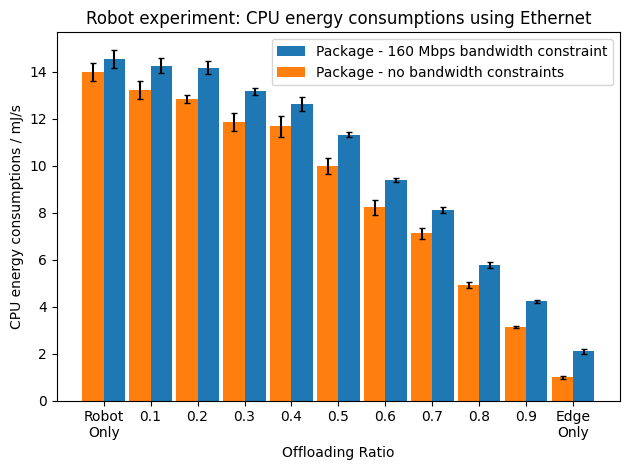
\includegraphics[width=\linewidth]{figures/experiment/real_robot/eth/cpu_energy_consumption.png}
    \caption{Real-robot experiment: CPU energy consumption using Ethernet}
    \label{fig:real_robot_experiment:eth_cpu_energy_consumption}
\end{figure}

% Figure for network bandwidth
\begin{figure}
    \centering
    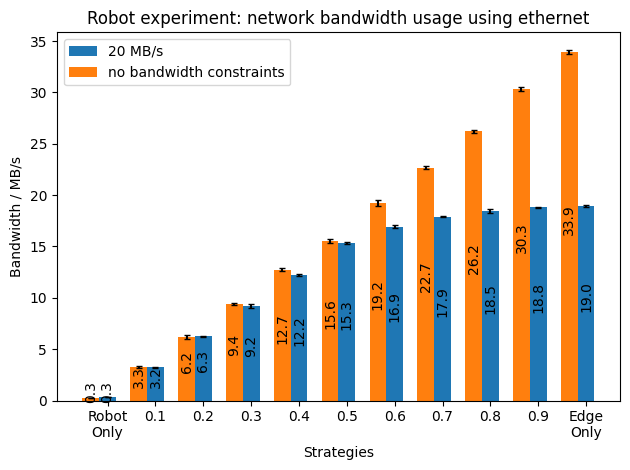
\includegraphics[width=\linewidth]{figures/experiment/real_robot/eth/bandwidth.png}
    \caption{Real-robot experiment: network bandwidth usage using Ethernet}
    \label{fig:real_robot_experiment:eth_bandwidth}
\end{figure}

\subsection{Wi-Fi}

The figures (TODO: add a figure here) and (TODO: add a figure here) present the results of the experiments using \gls{wifi}. 
